%%%%%%%%%%%%%%%%%%%%%%%%%%%%%%%%%%%%%%%%%%%%%%%%%%
%%%            TITLE: Video Game Loot Boxes and Gambling   
%%%
%%%            AUTHOR: Kevin Duong
%%%
%%%%%%%%%%%%%%%%%%%%%%%%%%%%%%%%%%%%%%%%%%%%%%%%%%
\errorstopmode

\documentclass[11pt]{article}
\usepackage{fullpage}


% wider spacing
\renewcommand\baselinestretch{1.5}

% Use the postscript times font!
\usepackage{times}
\usepackage{latexsym}
\usepackage{graphicx}
\usepackage{theorem}
\usepackage{latexsym}
\usepackage{caption}
\usepackage{tablefootnote}

\usepackage[utf8]{inputenc}
\usepackage[TS1,T1]{fontenc}
\usepackage{fourier,erewhon}
\usepackage{amssymb, amsbsy}
\usepackage{array, booktabs, longtable}
\usepackage[x11names, table]{xcolor}
\usepackage{caption}
\usepackage[normalem]{ulem}
\useunder{\uline}{\ul}{}




%table formatting provided by https://www.overleaf.com/learn/latex/Tables

\long\def\ignore#1\endig{}      % ignore (comment out) text thru \endig

% set up labeled statements or paragraphs that can be referenced by number.

\theorembodyfont{\rmfamily}
\newtheorem{thm}{Theorem}{\bfseries}{\rmfamily}
\newtheorem{eg}[thm]{Example}{\bfseries}{\rmfamily}
\newtheorem{defn}[thm]{Definition}{\bfseries}{\rmfamily}


%%%%%%%%%%%%%%%%%%% abbreviation-type macros %%%%%%%%%%%%%%%

\newcommand\genref[2]{#1~\ref{#2}}
\newcommand\sectref[1]{\genref{Section}{#1}}
\newcommand\figref[1]{\genref{Fig.}{#1}}
\newcommand\tblref[1]{\genref{Table}{#1}}
\newcommand\defnref[1]{\genref{Def.}{#1}}
\newcommand\thmref[1]{\genref{Theorem}{#1}}
\newcommand\egref[1]{\genref{Example}{#1}}
\newcommand{\eqnref}[1]{Eq.~\ref{#1}}

\newcommand{\clause}[1]{\left[ #1 \right]}

\newcommand{\set}[1]{\left\{#1 \right\}}      % argument is a set; put in { }.

\newcommand\textsquare{\raisebox{3pt}{\framebox[6pt]{\rule{0pt}{0.1pt}}}}

%%%%%%%%%%%%%%%%%%% END abbreviation-type macros %%%%%%%%%%%%%%%
\begin{document}

\title{Video Game Loot Boxes and Gambling}
 
\author{Kevin Duong\\
CMPS132W\\
keduong@ucsc.edu}

\date{}
 
\maketitle 
 
\begin{abstract}

Recent research has found strong links between certain reward mechanisms 
found in many of the most popular video games and indications of problem gambling. 
These reward mechanisms, colloquially referred to as loot boxes,
 vary in specific details but all typically share the same principle of 
being a virtual item containing randomized items. 
While these items have existed in some form as loot systems in games
released early as 2004, recent presentation of loot boxes in popular games 
has sparked many to bring into question the ethics and legality of these items. 
Arguments have been made that loot boxes can be interpreted as a form of gambling, 
especially in the case where the rewards can be cashed out for real world currency.
This paper aims to evaluate the relevancy of loot boxes by giving a formal 
definition to loot boxes, reviewing previous studies linking loot boxes to gambling,
and exploring legislation pertaining to the regulation of loot boxes.
\end{abstract}
 
 
 
\section{Introduction}\label{intro-sect}

The phenomenon of loot boxes swept across the gaming community 
in late 2017, eventually finding its way into the mainstream media and national
news \cite{pu_28AD}. The news coverage showcased this prominent mechanic of many video games 
that as whole generated an estimated \$30 billion in 2018, and is projected to surpass \$50 billion
by 2022 \cite{juniper2018}. Despite the vigorous growth of the video game industry due to loot boxes, 
most of the news coverage consisted of comparing loot boxes to gambling. Many referenced to 
the lack of regulation pertaining to loot boxes as well as the numerous studies 
concluding that loot boxes psychologically emulated gambling \cite{Drummond2018} as 
showed significant links with problem gambling \cite{zd01}. Studies began to link loot boxes
to motivations for adolescents to gamble \cite{zendle_meyer_over_2019}, and eventually the issue
of loot boxes made its way to the debate of nations globally. Some countries like Belgium and
Netherlands outright banned the sale of loot boxes in gaming, while in the US multiple pieces of legislation
have been proposed in efforts to regulate loot boxes \cite{yin-poole_2018} . 


\section{Loot Box Definition, Background, and Relevancy}\label{lootbox-dbr-sect}
To better understand the dynamic between loot boxes and gambling, we will first
try to define what a loot box is. The term \emph{loot box} is a general term and has
been likened to the notion of opening trading card packs, or baseball cards. For
the purposes of this paper we will restrict the definition of the loot box to the 
definition provided by Schwiddessen and Karius:

\begin{defn}\label{lootbox-defn}
"The term ‘loot box’, also known as ‘loot crate’ or ‘prize crate’ and other names,
typically refers to a consumable virtual item which can be redeemed to receive a
randomized selection of further virtual items, ranging from simple customization
options for a player’s game character, to game-changing equipment such as weapons,
armor, virtual currency, additional skills and even completely new or exclusive
characters… Loot boxes can be differentiated in two categories: Those dropping
cosmetic items (the latter… often referred to as ‘skins’) and those generating items
relevant for gameplay progress." \cite{article}
\end{defn}

We will also be referring to video game \textit{micro-transactions} through the following definition:

\begin{defn}\label{mt-defn}
"[A microtransaction] commonly refers to a business model… where users can
purchase virtual goods via micropayments… Microtransactions (i.e. premium content)
may include downloadable content such as story extensions (so called ‘DLCs’),
additional play time, levels, new maps, virtual currency, weapons, armor, characters
or cosmetic items to customize the player’s character or items. The player pays…
either directly with real world currency or with some form of fantasy virtual currency
(e.g. gold). The latter is typically earned during gameplay or can (often alternatively)
be purchased with real world money." \cite{article} 
\end{defn}


\subsection{Loot Box Design} \label{lootbox-design-sect}
Loot boxes vary in design over many different video games, but most share a few key features: 
\begin{itemize}
   \item Presentation of a digital box, container, or pack with randomized contents.
   \item The chances of getting any certain item among the randomized content is fixed, leading to low 
   chance rate item to be highly desired.
   \item Opening of the loot box is dramatized, i.e. an animation is played to delay the opening 
   of the box to build anticipation similar to the spinning of a slot machine. This is 
   to motivate future purchases, explained in  \sectref{psych-design-sect}.
\end{itemize}
Loot boxes can be obtained in different ways over different games, being 
obtainable through game progression (e.g. leveling-up), direct purchase, or sometimes both.
Consumers typically pay real-life currency in exchange for loot boxes (or for virtual
currency which is then traded for loot boxes) which are then opened. The contents are 
randomized, though the odds of getting any particular item in the box are often fixed. This
makes room for categorization of the loot box contents in tier lists based on drop rate, 
typically amongst some structure of basic, rare, and unique tiered loot. Loot boxes also vary in 
the amount of items given in each opening, with some games like \textit{Counter-Strike: Global
Offensive} only giving one item per box opening, while other games like \textit{Overwatch} give
three. Games with loot boxes that offer multiple items typically have the 
caveat of containing at least one item of better quality to incentivize consumers to buy them \cite{McCaffrey2019}.
Some games have options to recycle items for virtual currency to either buy more loot
boxes, or directly purchase the desired item. This feature is intentionally not accessible 
in most games to make obtaining items more difficult and therefore encourage loot box purchases. 


\subsection{Loot Box History}\label{lootbox-hist-sect}
The origins of Loot Boxes can be traced back to the early 2000's, with the emergence of a new
genre of gaming known as \textbf{free-to-play} (F2P). These games were to 
available on the internet 
at no cost, but had provisions in-game which strongly motivated users to spend
real-life currency to purchase in-game content \cite{zendle_meyer_over_2019}.
 This format of releasing games 
proved to be effective in raising profits, with the Chinese game \textit{ZT Online} reporting
in 2007 monthly revenues of over \$15 million USD \cite{koo}. Game developers 
realized that it was more profitable to release a free game riddled with micro-transactions
 (see \textbf{ \defnref{lootbox-defn}}) and optional premium content rather than 
 with releasing a full game set at a fixed price. 
Mobile developers followed shortly after, with Japanese based company 
GungHo releasing free mobile game \textit{Puzzle \& Dragons}, which in 2014 became the
 first mobile game to earn more than \$1 billion USD \cite{jordan_2014}. 
 Non-F2P game developers soon joined in on adding additional 
 purchasable content to their games, realizing they could release paid title games 
 that also include micro-transactions. 
 One of the first notable instances of this is in 2016 when US-based company 
 Blizzard released \textit{Overwatch} at a base price of \$60 USD, but also 
 included the option of purchasing loot boxes containing purely cosmetic items. 
This multi-layer payment system found major success globally,
with Blizzard reporting \$1 billion USD in \textit{Overwatch's} first year \cite{juniper2018}.
Eager to match \textit{Overwatch's} success,
 other game developers began releasing paid titles with loot boxes. Some even
 added new loot box systems in their already existing games, such as with Riot Games's 
 \textit{League of Legends}, released in 2009 but offering loot boxes in 2016 \cite{juniper2018}.
 To better understand why loot boxes so prevalent in gaming and appeal to consumers,
we will discuss the psychology of loot boxes in \sectref{lootbox-psych-sect}.


\subsection{Loot Box Controversy}\label{lootbox-contr-sect}
Loot boxes have been adapted by different video game developers to best fit their own business models. 
However in 2017, EA Games would be known for releasing the title with the most controversial usage of loot boxes
in the history of the video game industry. \textit{Star Wars Battlefront 2} was released in late 2017, 
including a return of the popular feature of \emph{star cards},
items that give players new abilities and skills. The controversy arose when these items 
were restricted to being exclusive loot box rewards, meaning you could no longer
pay for these bonus items but rather pay for a chance at them \cite{zendle_meyer_over_2019}. Further 
complications with multiple in-game currencies would lead to the startling  
conclusion that you could pay for multiplayer advantages \cite{zendle_meyer_over_2019}.
This essentially made the game "pay to win", meaning gameplay would cater to the portion of consumers
willing to pay more. After public backlash and a hit to overall market value, 
EA games was resorted to temporarily disabling all microtransactions from the game all together \cite{McCaffrey2019}. 
Similar microtransaction strategies were utilized in 2K Sports' \textit{NBA 2K18} and Monolith Production's
\textit{Middle-Earth: Shadow of War}, but both equally met with consumer backlash \cite{McCaffrey2019}.
The infamy of loot boxes would lead to many to claim that loot boxes emulated gambling,
and question the purpose of loot boxes in video games. We will explore some studies 
conducted on loot boxes in  \sectref{gambling-sect}.



\section{Psychology of Loot Boxes}\label{lootbox-psych-sect}
The psychology behind loot boxes is designed to the appeal consumers.
Marketing strategies used by video game publishers have the same goal: to sell
as many loot boxes to consumers as possible. Fogg's Behavior Model explains 
how consumers are typically motivated, while
Eyal's Hooked Model and the \emph{gamblers' fallacy} provide insight on
why consumers return for more in the future.


\subsection{Behavioral Design of Loot Boxes}\label{psych-design-sect}
The appeal of buying loot boxes lies in the marketing strategies of game
publishers. To make the boxes enticing to consumers, various methods 
are employed to motivate purchases. These motivations are referred to as triggers
\cite{mei_mei_2018}, taking various forms such as advertisements on the internet
 or messages that show up on game loading screens. With these triggers, the transaction
model for loot boxes are typically set up to be as simple and user-friendly as 
possible. This makes it easy for consumers to enter in payment information and 
receive their loot boxes in a promptly. This is described in Fogg's 
Behavior model, shown in \figref{behavior-model-fig}.
\begin{figure}
\centering
\begin{picture}(550,200)
\put(0,0){\scalebox{.4}{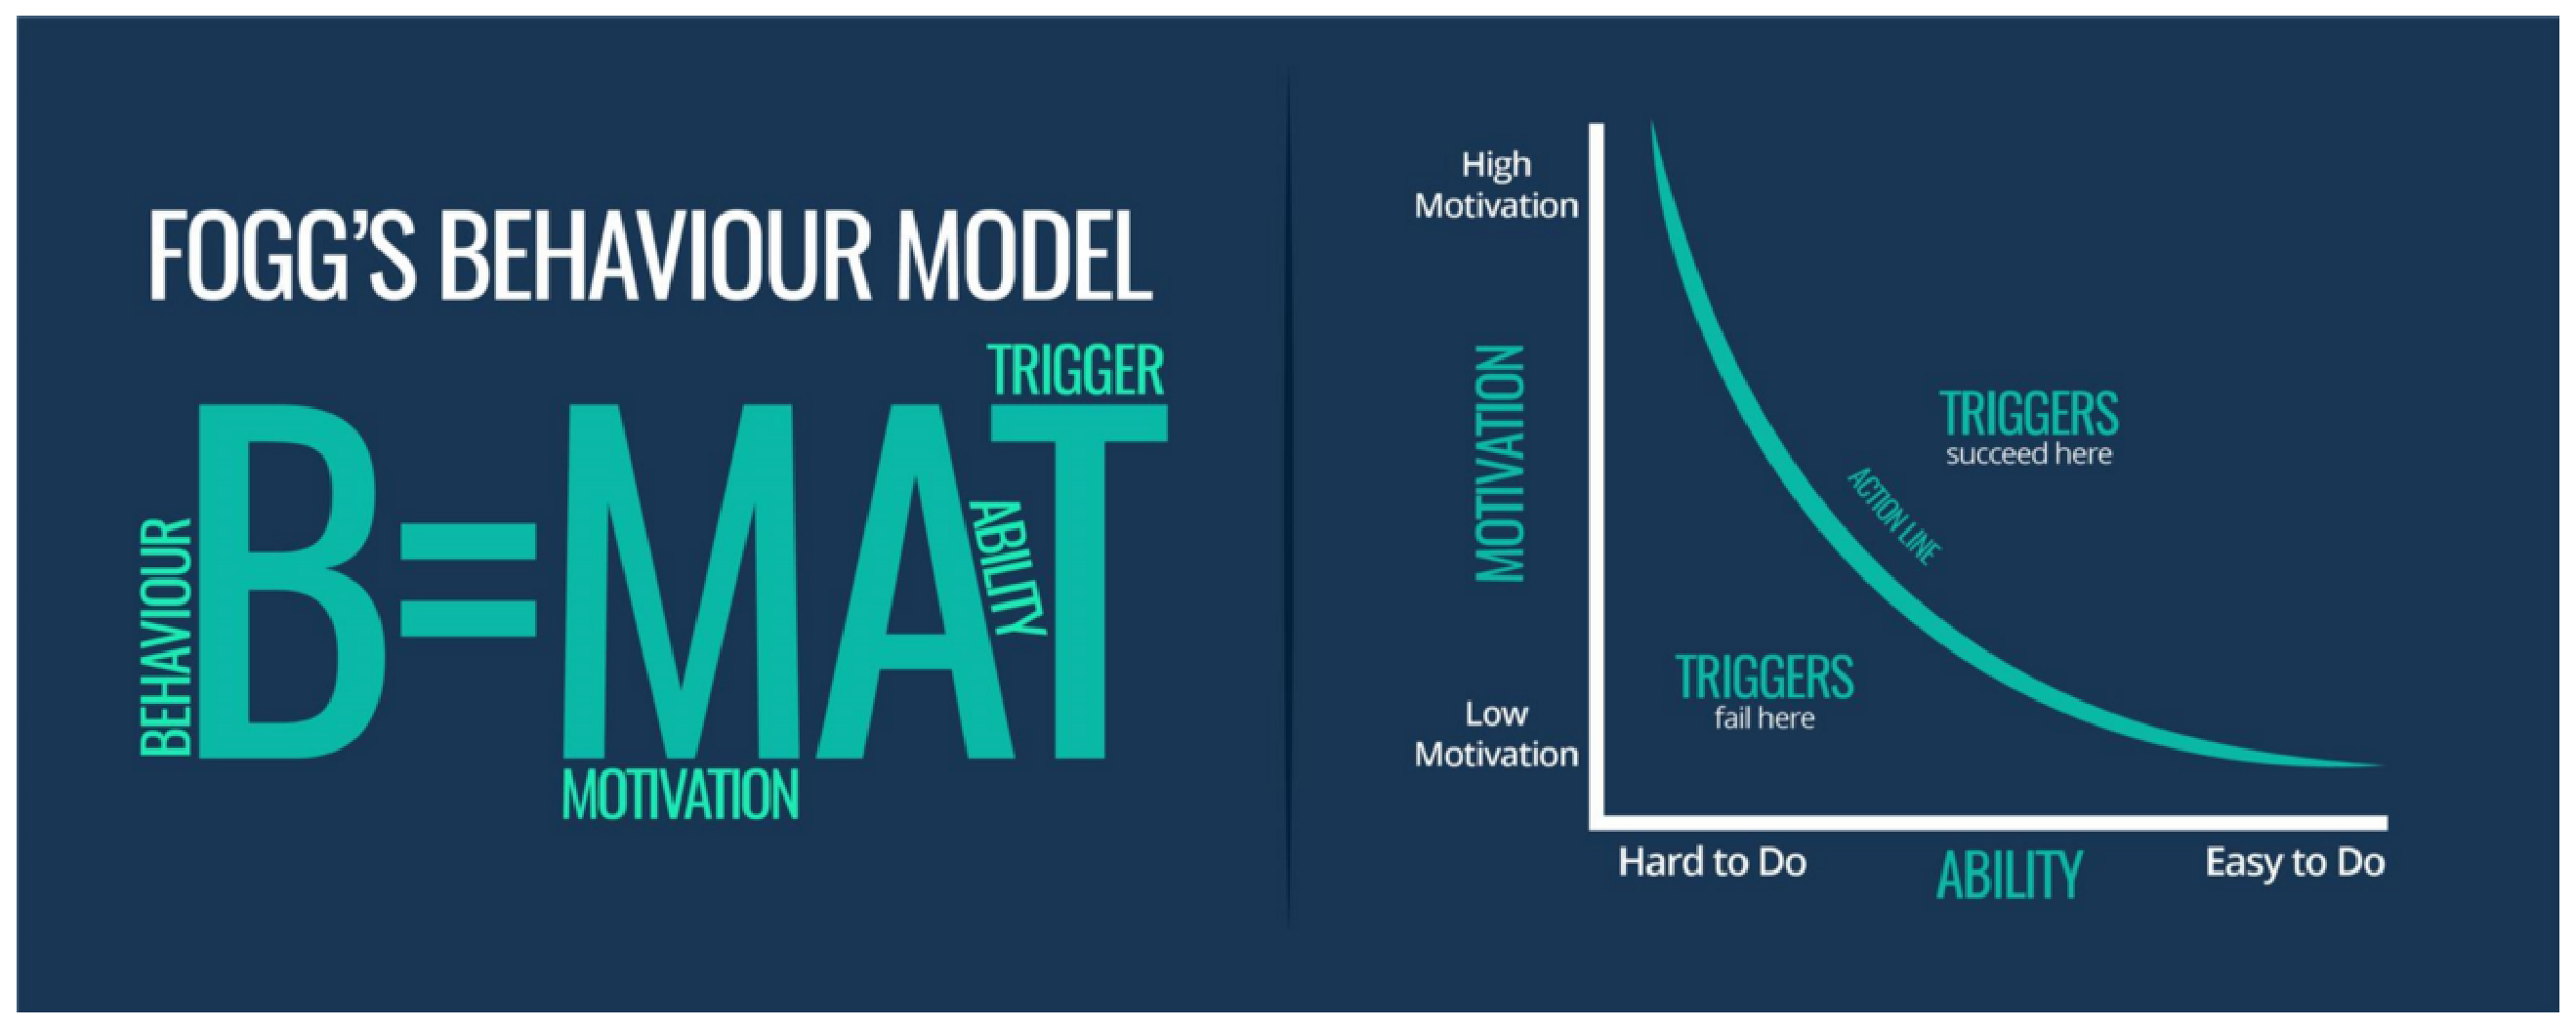
\includegraphics{behavior-model.eps}}}
\end{picture}
\caption{Fogg's behavior model as illustrated by Growth Engineering.}
\label{behavior-model-fig}
\end{figure} 
The equation states that a consumer's behavior B is a function of that consumer's motivation M, 
their ability in performing that behavior A, and whether a trigger is present T.  
If one of the variables is missing or lacking, users will fall below the theoretical action line, 
thus not performing the action \cite{mei_mei_2018}. 
In addition to this, Eyal's Hooked model shown in \figref{hooked-model-fig} describes
how consumers end up returning to make future purchases. It is described in four steps:
\begin{enumerate}
   \item Trigger: An internal/external trigger is exposed to consumers which grabs the
   interest or curiosity of consumers, e.g. advertisements.
   \item Action: A means of action is offered to consumers to respond to the trigger,
   in this case purchasing loot boxes.
   \item Variable Reward: Varying rewards are given out to the consumer,
   usually appealing the consumer's excitement by adding a delay before
   giving the reward, e.g. building anticipation with the spinning on a slot machine.
   This feeling of anticipation builds the foundation for the next stage.
   \item Investment: Manipulation of the product to motivate consumers to 
   use the product again.
\end{enumerate}
\begin{figure}
\centering
\begin{picture}(300,275)
\put(0,0){\scalebox{.50}{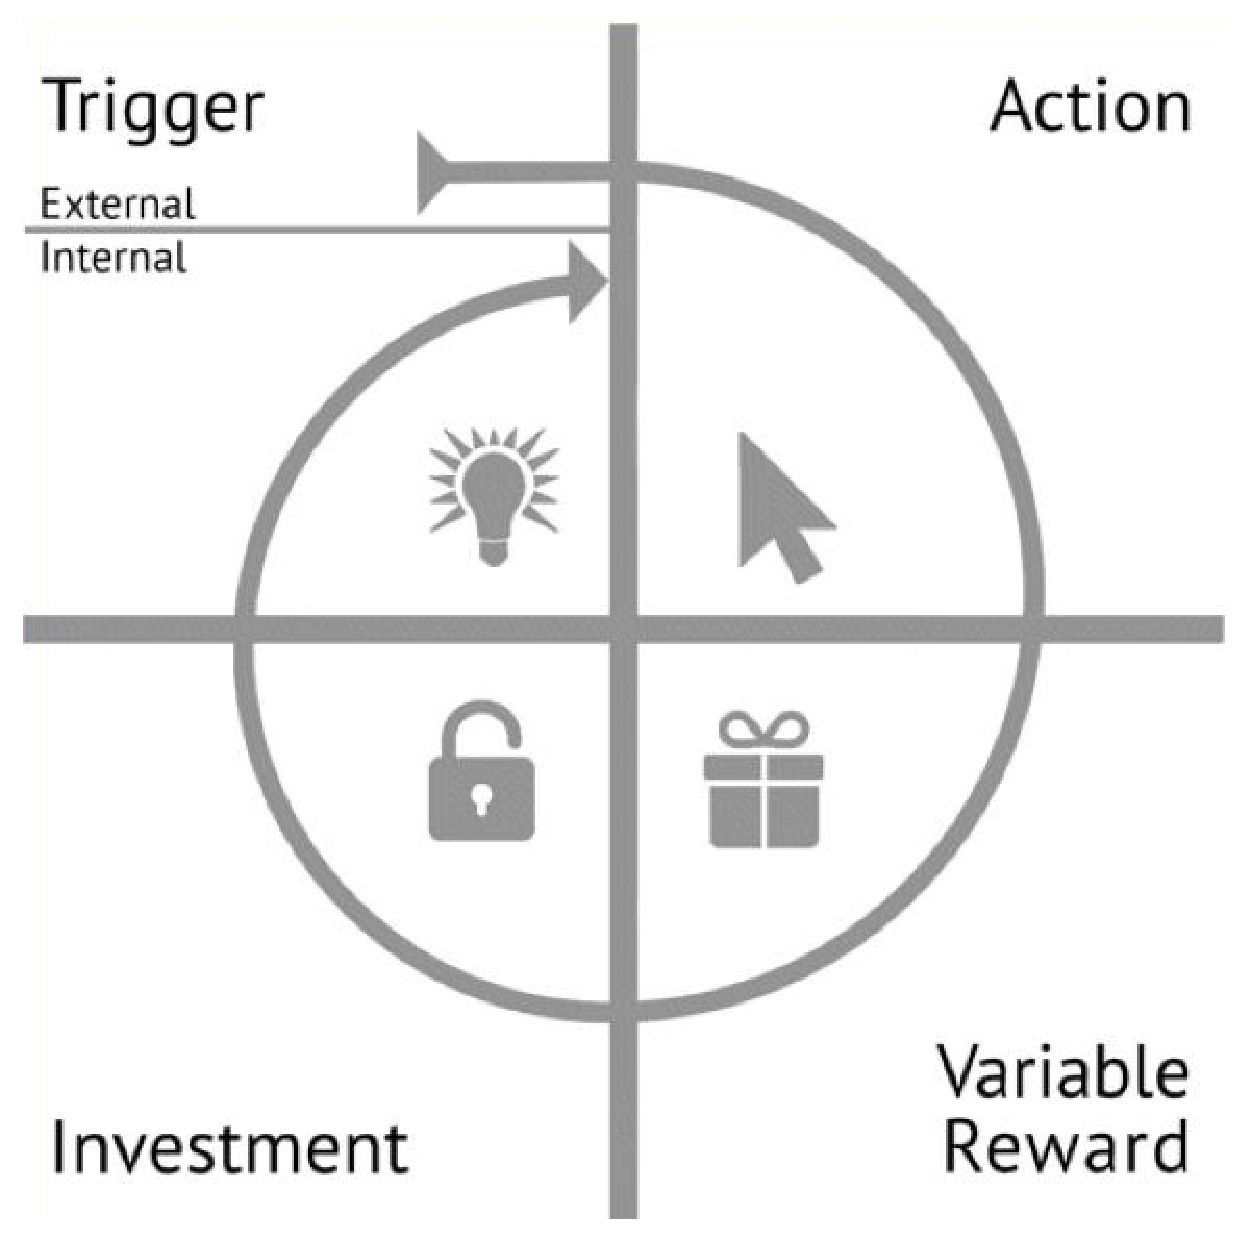
\includegraphics{hooked-model.eps}}}
\end{picture}
\caption{The Four Steps of the Hooked Model by Nir Eyal. \cite{hooked2014}}
\label{hooked-model-fig}
\end{figure} 
Eyal's hooked model visualizes business design with the purpose of enticing consumers
to buy into a product they typically would not necessarily feel the need to purchase, 
as well as motivate them to to make repeat purchases in the future. In this sense,
the ideal scenario for game developers is to have consumers fall into the hooked model
and continue to purchase loot boxes. The repeated purchases of loot boxes can
lead to addiction as a direct result of excessive spending in order to get a desired
outcome, a condition akin to gambling addiction \cite{zd01}.

\newpage
\subsection{Gambler's Fallacy}
In some instances, gamers that open loot boxes with the intent of getting specific desired items (i.e. 
\emph{star cards} in \sectref{lootbox-contr-sect}) but fail to get them may feel 
inclined to continue to spend until that item is achieved. These gamers may be motivated
by the fact that since the first few boxes don't have their desired item, surely the 
next few should contain it. This mistaken belief that if things happen more frequently 
than usual in a certain time period then it will happen less often in the future (or vice
versa) is known as the Gambler's Fallacy (or Monte Carlo Fallacy) \cite{kenton_2019} . To better visualize
this, we will use the example of consecutive coin tosses. The outcome of different
tosses are independent, and the odds of getting heads is \(\frac{1}{2}\). Getting two heads 
in two tosses would be \(\frac{1}{4}\), three in three tosses would be \(\frac{1}{8}\), and
so on. In general, if \(A_i\) is the event where toss \textit{i} of a fair coin results 
in heads, then :
\begin{equation}
  Pr\Bigg(\bigcap_{i=1}^{n}A_i\Bigg)  = 
  \prod_{i=1}^{n} Pr\big(A_i\big) =
  \frac{1}{2^n}.
\end{equation} 
If after three tosses with all landing heads, another toss resulting in heads would
be a run of four successive head tosses. The probability of flipping four heads in a row
is \(\frac{1}{16}\), which could form the mistaken belief that the next toss would end in
tails instead of heads. The event of four successive head tosses has the exact same 
probability of the event of three successive head tosses followed by tails (\(\frac{1}{16}\)). 
A run of four successive head tosses is improbable at about 6\%, 
but it is crucial to recognize that probability only applies before the first coin is tossed. 
The probabilities of three successive tosses are equal to 1, thus the outcome of the next toss 
is independent. The idea that the fourth toss is more likely to be tails due
to an improbable run of heads epitomizes the gambler's fallacy, and perhaps explains
how so many individuals end up spending so much money on loot boxes.
When the spending parallels that of addiction, concerns of loot boxes being 
too similar to gambling are raised. We will discuss this in \sectref{gambling-sect}.



\section{Loot Boxes and Gambling}\label{gambling-sect}
With the excessive usage of loot boxes in video games along with instances of questionable designs, 
claims were made that the practice of using loot boxes was too similar to gambling \cite{pu_28AD}. 
As a result, many reviews and studies were done to study the ethics behind
loot boxes. This section will compare loot boxes and gambling as defined by Griffiths' five characteristics 
of gambling \cite{Drummond2018}, as well explore the findings of multiple surveys that linked loot boxes to 
problem gambling. 

\renewcommand\baselinestretch{1.2}
\begin{table}
\footnotesize 
\caption{Loot Boxes in video game titles, defined by Grifffiths' five gambling principles \cite{Drummond2018}}. \label{lootbox-table}
\begin{tabular}{l*{6}{c}r}
Title                                               & ESRB Rating\footnote   &Purchasable  &Chance Involved   &Advantage    &Cash-out \\
\hline
Apex Legends                               &13+                 &\checkmark  &\checkmark              &                  & \\ \hline
Assassins Creed Origin                 &17+                  &\checkmark  &\checkmark             &\checkmark   &\\ \hline
Battlefield 1                                  &17+                  &\checkmark  &\checkmark             &                   & \\ \hline
Call of Duty: WWII                      &17+                  &\checkmark  &\checkmark              &\checkmark  & \\ \hline
Counter-Strike: Global Offensive &17+                 &\checkmark  &\checkmark              &                   &\checkmark  \\  \hline
Destiny 2                                      &13+                  &\checkmark  &\checkmark             &                   & \\ \hline
FIFA 17                                        &E                      &\checkmark  &\checkmark              &\checkmark   &\checkmark  \\ \hline
FIFA 18                                        &E                     &\checkmark  &\checkmark                &\checkmark  &\checkmark  \\ \hline
For Honor                                     &17+                &\checkmark  &\checkmark                &\checkmark  & \\ \hline
Fortnite                                        &13+                 &\checkmark &\checkmark                &\checkmark  & \\ \hline
Forza Motorsport 7                      &E                     &\checkmark  &\checkmark                &\checkmark  & \\ \hline
Gears of War 4                            &17+                &\checkmark  &\checkmark                &                  & \\ \hline
Hearthstone                                &13+               &\checkmark   &\checkmark                &\checkmark    & \\ \hline
Halo Wars 2                                 &13+               &\checkmark   &\checkmark                &\checkmark   & \\ \hline
Injustice 2                                   &13+               &\checkmark   &\checkmark                 &\checkmark   & \\   \hline
Lawbreakers                               &17+               &\checkmark   &\checkmark                  &                  &\\ \hline
League of Legends                     &13+               &\checkmark   &\checkmark                  &                  & \\ \hline
Madden NFL 17                           &E                   &\checkmark   &\checkmark                  &\checkmark  & \\ \hline
Madden NFL 18                           &E                   &\checkmark   &\checkmark                  &\checkmark  &\checkmark  \\ \hline
Mass Effect 3                              &17+              &\checkmark   &\checkmark                 &\checkmark  &\checkmark  \\ \hline
NBA 2K18                                    &E                   &\checkmark   &                                &                   & \\ \hline
Need for Speed Payback            &13+              &\checkmark   &\checkmark                 &\checkmark   & \\ \hline
Overwatch                                  &13+              &\checkmark   &\checkmark                 &                  & \\ \hline
PlayerUnknown's Battlegrounds &13+              &\checkmark    &\checkmark               &                  &\checkmark \\ \hline
Puzzle \& Dragons                      &E                   &\checkmark  &\checkmark                  &\checkmark    & \\ \hline
Rainbow Six: Siege                     &17+               &\checkmark   &\checkmark                 &                  & \\ \hline
Rocket League                           &E                   &\checkmark   &\checkmark                 &                   & \\  \hline
Star Wars Battlefront II             &13+              &                    &\checkmark                &\checkmark    & \\ \hline
ZT Online                                    &13+              &\checkmark   &\checkmark                 &\checkmark    & \\ \hline

\end{tabular} 
\newline

\end{table}
\renewcommand\baselinestretch{1.5}


\subsection{Gambling Specifics} \label{griffith-gamble-sect}
To see the similarities between loot boxes and gambling, we can refer to Griffiths' 
five principles \cite{Drummond2018} to distinguish gambling activities: 
\begin{enumerate}
   \item The exchange of money or valuable goods.
   \item An unknown future event determines the exchange.
   \item Chance plays partly in the outcome of the exchange.
   \item Opting out of the exchange avoids losses.
   \item One party clearly wins at the cost of the other party losing.
\end{enumerate}
Drummond includes a sixth principle \cite{Drummond2018}: an ability to 
exchange winnings into real-world currency, or an option to cash-out. With these 
characteristics we can assess the validity behind the claim that loot boxes
emulate gambling. Drummond observed the 22 games from 2016-2017 
which included loot boxes, which is supplemented by individual research 
for 2018 games in \tblref{lootbox-table}. The criteria of the table reflects the six characteristics
with the exclusion of the ability to opt out to avoid losses (since this would
obviously apply to each game), in order to better compare gambling and 
loot boxes. Seventeen out of the listed 29 games (58\%) cover all 5 of Griffiths' 
gambling characteristics, with 6 of these 17 games having an option to 
convert winnings into real-world currency. While it is important to note
that these 6 games have provisions in their terms of service that
explicitly prohibit the sale or trade of in-game currencies
 \cite{Drummond2018} , the actual items received are easily
  sold/exchanged through online marketplaces, such as with 
  \textit{Counter Strike: Global Offensive}, which was worth a reported
\$10 billion USD through the sale/exchange of in-game cosmetic items 
earned in loot boxes \cite{juniper2018}. With such prevalence in the 
video game industry, the loot box can be manipulated in many ways 
by video game developers, and as seen many of these instances
are akin to gambling.


\subsection{Loot Boxes and Problem Gambling}\label{gambling-survey-sect}
Zendle and Cairns \cite{zd01} and later Zendle, Carins, McCall, and Barnett \cite{zmbc} 
conducted studies on whether or not loot boxes could be correlated 
with instances of problem gambling. In the first study, 
Zendle and Cairns interviewed 7,422 adult gamers to assess the
link between the amount of money spent loot boxes to the degree
of their gambling addiction, seen in \figref{problem-gambling-survey-1-fig}. 
The study noted that the link was stronger between 
money spent on loot boxes than when compared to the link with buying other
in-game items with real-world money. This finding suggests that the gambling-like
 features of loot boxes can be responsible for the observed trend 
between loot boxes and problem spending. While it is unclear whether 
this is an implication that loot boxes are a gateway to problem gambling or if 
loot boxes simply appeal to problem gamblers, it does clearly highlight a strong
link between problem gambling and the purchase of loot boxes. 
\begin{figure}
\begin{picture}(200,275)
\put(0,0){\scalebox{.88}{\includegraphics{problem-gambling-survey-1.eps}}}
\end{picture}
\caption{Amount of money put into loot boxes monthly versus problem
gambling severity. \cite{zd01}}
\label{problem-gambling-survey-1-fig}
\end{figure}
A follow up survey done on 1,200 adult individuals determined that 
when judging gamers who engage in unpaid openings of loot boxes
(free boxes) against those who do paid openings, those who pay to open 
boxes were much more likely to have a higher problem gambling severity
\cite{zmbc}. As seen in \figref{problem-gambling-survey-2-fig}, those 
who paid for loot boxes had on average double the severity in 
problem gambling to those who only opened free boxes. The survey continues
to note that while some loot box features may mitigate some of the risk of 
higher problem gambling severity, the main conclusion is that the
exchange of real-life currency for virtual content is the main driving
force for problem gambling.
\begin{figure}
\begin{picture}(200,225)
\put(0,0){\scalebox{1}{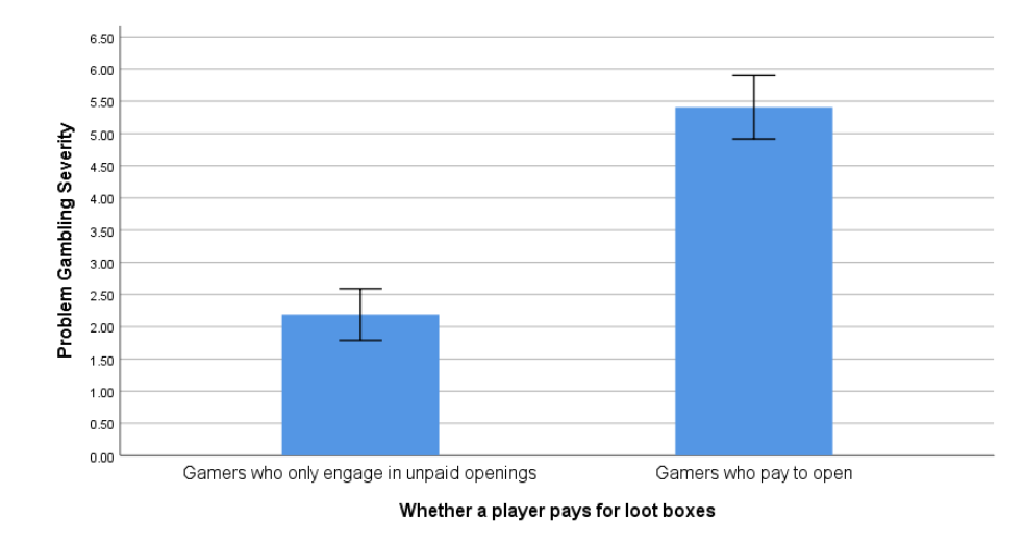
\includegraphics{problem-gambling-survey-2.eps}}}
\end{picture}
\caption{Problem Gambling severity versus opting in or out of paying for
loot boxes in adults. \cite{zmbc}}
\label{problem-gambling-survey-2-fig}
\end{figure}


\newpage
\subsection{Adolescent Gambling}
Zendle, Meyer, and Over \cite{zendle_meyer_over_2019} surveyed 1155 adolescents
within the age of 16-18 to gauge the relationship between loot box spending and
problem gambling. This survey was done after the surveys reviewed in 
\sectref{gambling-survey-sect} in order to compare the severity in adults
versus in adolescents. The results in \figref{adolescent-1-fig} showed that
the link between loot box spending and problem gambling was more
than twice of that observed in adults \cite{zendle_meyer_over_2019}. 
Furthermore the results found direct correlation between higher
loot box spending with more serious problem gambling 
classification, observable in \figref{adolescent-2-fig}. These
findings not only suggest that adolescents are at higher risk than adults
to establish problem gambling habits when spending more money
on loot boxes, but also show implications that video game companies
are profiting from developing problem gambling in adolescents. 
The stronger link between problem gambling and loot boxes 
in adolescents can also be attributed as a byproduct of peer
pressure, with young gamers giving their best efforts to match
the monetary spending of their peers \cite{Wilber2006}. 
Because of easy accessibility of gambling-like activities,
such as buying loot boxes, gambling can seem more leisurely.
This generalizes gambling to be more widely accepted, even
when done by adolescents \cite{cv12}. This overall has serious 
implications on the morals of the video game industry, and also 
puts weight on the political sector to oversee much needed regulation
and policies on gambling-like loot boxes. These policies will 
be discussed in \sectref{lootbox-law-sect}.
\begin{figure}
\begin{picture}(200,240)
\put(0,0){\scalebox{.78}{\includegraphics{adolescent_survey_2.eps}}}
\end{picture}
\caption{Trends between buying loot boxes and problem gambling
in adolescents.
 \cite{zendle_meyer_over_2019}}
\label{adolescent-1-fig}
\end{figure}
\begin{figure}
\begin{picture}(200,220)
\put(0,0){\scalebox{.8}{\includegraphics{adolescent_survey_1.eps}}}
\end{picture}
\caption{Trends between loot box spending and problem gambling classification 
in adolescents.
 \cite{zendle_meyer_over_2019}}
\label{adolescent-2-fig}
\end{figure}


\newpage
\subsection{Regulation}\label{lootbox-law-sect}
Given the infamy of loot boxes, discussions on possible regulation made 
their way into political circles around the world. Through independent review,
as well as consideration of funded case studies \cite{McCaffrey2019}, countries have 
already started to take action in determining the extent of loot box influence. 
Global discussions focused on two different issues pertaining to loot boxes: 
gambling and transparency. If loot boxes were found to be gambling, then they would 
regulated as such. In terms of transparency, concerns on consumer exploitations 
were made given instances of deceptive or predatory marketing practices, especially 
when in consideration of presentation towards children \cite{McCaffrey2019}.
These two issues have elicited different responses from different countries,
as presented in \tblref{legis-table}. The most extreme responses were by Belgium, Netherlands, 
and Japan who all determined loot boxes to be forms of gambling and banned 
the sale of gambling-based loot boxes in video games entirely. In countries with larger
populations of gamers, U.S., U.K., and China, loot boxes were found to
\textit{not necessarily} be gambling, though more investigation would be 
needed to make a formal decision \cite{McCaffrey2019}, 
leaving room open for possible legislation to pass.
In September 2018, gambling commissions from 15 European nations of 
Austria, the Czech Republic, France, Gibraltar, Ireland, Isle of Man, Jersey, Latvia, 
Malta, the Netherlands, Norway, Poland, Portugal, Spain, UK, 
as well as the state of Washington from the United States announced a 
collaborative effort to form legislation to better define the lines between
gambling and gaming \cite{kent_2018}. There have been efforts
for the video game industry to self-regulate through means of
updating guidelines and terms of services, though many of these
efforts have proven to be ineffective \cite{McCaffrey2019}.


\renewcommand\baselinestretch{1}
\begin{table}[]
\caption{Loot Box legal opinion and regulation by country \cite{McCaffrey2019}}
\label{legis-table}
\begin{tabular}{|l|l|l|} \hline
\textbf{Region}                                                      & \textbf{Legal Opinion or Action}                                                                                                                                                                                                                                                 & \textbf{Current Policy}                                                                                                                                              \\ \hline
Australia                                                            & Loot Boxes might be gambling                                                                                                                                                                                                                                                     & Pursing future investigation                                                                                                                                         \\ \hline
Belgium                                                              & Loot Boxes are gambling                                                                                                                                                                                                                                                          & Banned loot boxes                                                                                                                                                    \\ \hline
China                                                                & Loot Boxes might be gambling                                                                                                                                                                                                                                                     & \begin{tabular}[c]{@{}l@{}}(1) Draw rates must be accessible\\ (2) Ban purchase of loot boxes with \\ money\\ (3) Ban the trading of virtual\\ currency\end{tabular} \\ \hline
Denmark                                                              & Loot Boxes might be gambling                                                                                                                                                                                                                                                     & Cautioned parents                                                                                                                                                    \\ \hline
France                                                               & Loot Boxes might be gambling                                                                                                                                                                                                                                                     & Pursing future investigation                                                                                                                                         \\ \hline
Germany                                                              & \begin{tabular}[c]{@{}l@{}}Loot Boxes might be gambling, \\ can be harmful to children\end{tabular}                                                                                                                                                                              & Reviewing case-by-case                                                                                                                                               \\ \hline
Isle of Man                                                          & \begin{tabular}[c]{@{}l@{}}Loot Boxes might be gambling,\\ virtual currencies have value\end{tabular}                                                                                                                                                                            & Revising Gambling law                                                                                                                                                \\ \hline
Japan                                                                & Loot Boxes are gambling                                                                                                                                                                                                                                                          & Banned loot boxes                                                                                                                                                    \\ \hline
Netherlands                                                          & Loot Boxes are gambling                                                                                                                                                                                                                                                          & Banned loot boxes                                                                                                                                                    \\ \hline
New Zealand                                                          & Loot Boxes aren't gambling                                                                                                                                                                                                                                                       & No action                                                                                                                                                            \\ \hline
Singapore                                                            & Loot Boxes might be gambling                                                                                                                                                                                                                                                     & Pursing future investigation.                                                                                                                                        \\ \hline
South Korea                                                          & \begin{tabular}[c]{@{}l@{}}Loot Boxes might be gambling,\\ false advertising is dangerous\end{tabular}                                                                                                                                                                           & Threaten developers with fines                                                                                                                                       \\ \hline
Sweden                                                               & Loot Boxes aren't not gambling                                                                                                                                                                                                                                                   & Pursing future investigation.                                                                                                                                        \\ \hline
United Kingdom                                                       & \begin{tabular}[c]{@{}l@{}}Loot Boxes aren't gambling,\\ 3rd party markets for loot boxes\\ might be gambling\end{tabular}                                                                                                                                                       & \begin{tabular}[c]{@{}l@{}}(1) Cautioned parents\\ (2) Pursing future investigation\end{tabular}                                                                     \\ \hline
\begin{tabular}[c]{@{}l@{}}United States\\ (California)\end{tabular} & \begin{tabular}[c]{@{}l@{}}Loot Boxes might be gambling,\\ Bill proposed to mandate clear\\ packaging on games with \\ microtransactions.\end{tabular}                                                                                                                           & Bill allowed to die                                                                                                                                                  \\ \hline
\begin{tabular}[c]{@{}l@{}}United States\\ (Hawaii)\end{tabular}     & \begin{tabular}[c]{@{}l@{}}Loot Boxes might be gambling,\\ Bills proposed to: \\ (1) Restrict sale of games \\ with cash-out features to 21+ age limit.\\ (2) Demand draw rates for  loot boxes\\ (3) Games with gambling-like\\ features have to marked packaging.\end{tabular} & Bills allowed to die                                                                                                                                                 \\ \hline
\begin{tabular}[c]{@{}l@{}}United States \\ (Minnesota)\end{tabular} & \begin{tabular}[c]{@{}l@{}}Loot Boxes might be gambling\\ Bill proposed to:\\ (1) Games with gambling-like\\ features to have marked packaging.\\ (2) Restrict sale of games \\ with microtransactions to 18+ age limit.\end{tabular}                                            & Bill passed to a committee                                                                                                                                           \\ \hline
\begin{tabular}[c]{@{}l@{}}United States\\ (Washington)\end{tabular} & \begin{tabular}[c]{@{}l@{}}Loot Boxes might be gambling\\ Bill proposed to charge Gambling\\ Commission to investigate loot boxes.\end{tabular}                                                                                                                                  & \begin{tabular}[c]{@{}l@{}}Bill failed to advance through\\ committee\end{tabular}                                                                                   \\ \hline
\end{tabular}
\end{table}
%table generated by https://www.tablesgenerator.com/
\renewcommand\baselinestretch{1.5}



\newpage
\section{Recommendations}\label{recommend-sect}
Given the studies presented and reviewed in this paper, it is within reason 
to believe that loot boxes in some forms can constitute as gambling. To 
prevent the exploitation of consumers, as well as suppress gambling
in adolescents and children, more resources should be placed on 
defining a clear line between gaming and gambling. I would like to
present two options to explore: 
\begin{enumerate}
   \item Remove the option to buy loot boxes in video games with
   real-world currency.
   \item Task the Gambling Commission to thoroughly investigate
   the link between gambling and loot boxes and advise action.
 \end{enumerate}
 Drummond \cite{Drummond2018},
Zendle and Cairns \cite{zd01}, and Barnett and McCall \cite{zmbc},
have all built connections linking gambling and loot boxes. With the recent 
failures to pass legislation in the U.S. pertaining to loot boxes, 
video game developers should not be given the chance to push the limits of 
what is to be considered acceptable in terms of loot boxes. 
Video game loot boxes can still exist, but the problem lies in the 
option to purchase them with money. In-game items can still be
given monetary value since this is akin to online shopping, but the
process of opening loot boxes is too similar to gambling to allow the
flow of real-world money to be involved.
The Gambling Commission should also be involved with the joint effort 
from the 15 European countries, as well as the state of Washington, USA,
to establish guidelines for video game developers to follow and abide by.



\section{Conclusion}\label{conclusion-sect}
This paper has reviewed several studies conducted on both adult and 
adolescent gamers to verify the link between loot boxes and 
problem gambling. We have evaluated the psychological design
of loot boxes and how easily it can be manipulated to maximize 
profits, sometimes at the cost of predatory marketing practices 
at adolescents. With the current regulation, especially in the U.S.,
video game developers have taken the concept of loot boxes 
and manipulated them to best match their business models. 
The mechanic of loot boxes is a random reward system
and harmless on it's own, but becomes dangerous when made
available for exchange with real-world currency. In its modern
day form, the loot box has led to a need for a global discussion
between video game developers and gambling commissions 
on where the line is between gaming and gambling.


\bibliography{citelist}
\bibliographystyle{plain}

\end{document}



